\documentclass[tikz]{standalone}
\usetikzlibrary{mindmap}
% !TIKZEDT BOUNDINGBOX = -3 -3 8 5
\begin{document}
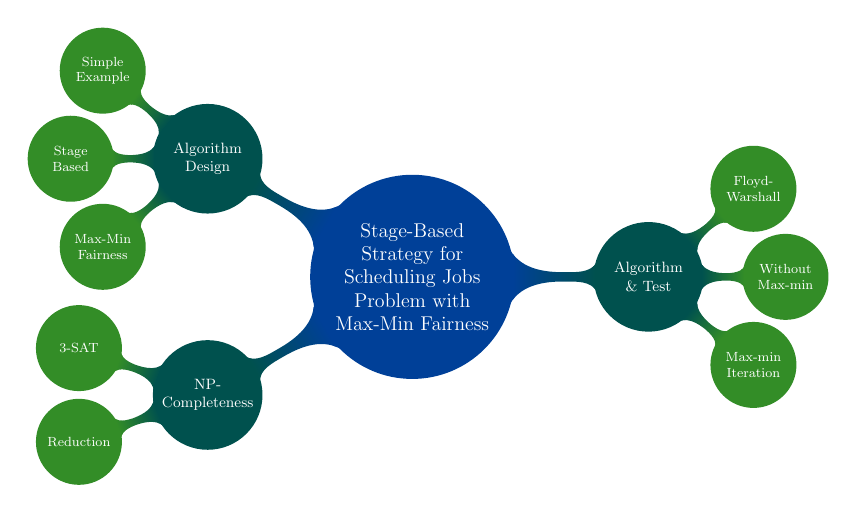
\begin{tikzpicture}[mindmap,concept color=cprimary,scale=0.6,every node/.style={scale=0.6},text=white]
\definecolor{cprimary}{RGB}{0,64,152}         %problue
\definecolor{csecondary}{RGB}{51,141,39}      %lightgreen
\definecolor{ctertiary}{RGB}{0,81,78}         %lightgray
\node [concept] {Stage-Based Strategy for Scheduling Jobs Problem with Max-Min Fairness}
child[concept color=ctertiary,grow=150] {
	node[concept] {Algorithm Design}
	child[concept,grow=140,concept color=csecondary] {node[concept] {Simple Example}}
	child[concept,grow=180,concept color=csecondary] {node[concept] {Stage Based}}
	child[concept,grow=220,concept color=csecondary] {node[concept] {Max-Min Fairness}}
	}
child[concept color=ctertiary,grow=210] {
	node[concept] {NP-Completeness}
	child[concept,grow=160,concept color=csecondary] {node[concept] {3-SAT}}
	child[concept,grow=200,concept color=csecondary] {node[concept] {Reduction}}
	}
child[concept color=ctertiary,grow=0] {
	node[concept] {Algorithm \& Test}
	child[concept,grow=40,concept color=csecondary] {node[concept] {Floyd-Warshall}}
	child[concept,grow=0,concept color=csecondary] {node[concept] {Without Max-min}}
	child[concept,grow=-40,concept color=csecondary] {node[concept] {Max-min Iteration}}
	};
\end{tikzpicture}    
\end{document}